\documentclass[12pt,a4paper]{article}
\usepackage[utf8]{inputenc}
\usepackage[german]{babel}
\usepackage[T1]{fontenc}
\usepackage{amsmath}
\usepackage{amsfonts}
\usepackage{amssymb}
\usepackage{graphicx}
\usepackage[left=3cm,right=3cm,top=3cm,bottom=3cm]{geometry}
\setlength{\parskip}{3mm}
\setlength{\parindent}{0cm}
\author{Maike Meier and Lasse Schuirmann}
\title{Messtechnik und Messdatenverarbeitung - Blatt 7}
\newcommand*{\blankpage}{
  \vspace*{\fill}
  \begin{flushright}
  \tiny THIS PAGE INTENTIONALLY LEFT BLANK.
  \end{flushright}
  \pagebreak
}
\begin{document}

\maketitle
\pagebreak

% See http://www.this-page-intentionally-left-blank.org/
\blankpage

\section*{Aufgabe 1}
\subsection*{1.1}
Um eine Ablösung des Sensors zu detektieren, kann der $\chi^2$-verteilung Anpassungstest durchgeführt werden.

Eine Voraussetzung für diesen Test ist, dass die Messwerte statistisch unabhängig sind und eine große Stichprobe vorhanden ist.

Der Test kann wie folgt durchgeführt werden:

\begin{enumerate}
\item Voraussetzungen sicherstellen
\item Klassen festlegen, Häufigkeiten $n_i$ bestimmen
\item Null- und Alternativhypothese aufstellen (ist normalverteilt/ist nicht normalverteilt)
\item Signifikanzniveau wählen
\end{enumerate}

\subsection*{1.2}
\scalebox{0.78}{
 \begin{tabular}{|r|c|c|c|c|c|c|c|c|}
 \hline
 Klasse & $\leq 35.0$ & $35.1 - 35.5$ & $35.6 - 36.0$ & $36.1 - 36.5$ & $36.6 - 37.0$ & $37.1 - 37.5$ & $37.6 - 38.0$ & $\geq 38.0$ \\
 \hline
 Anzahl $n_i$ & $4$ & $9$ & $16$ & $20$ & $16$ & $16$ & $6$ & $8$ \\
 \hline
 \end{tabular}}

\noindent
\begin{minipage}{0.6\textwidth}
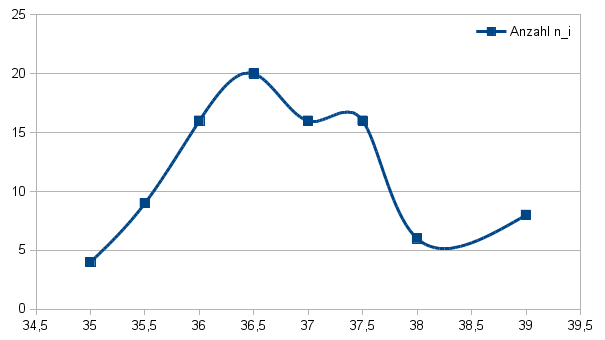
\includegraphics[scale=0.56]{1_2_diagram}
Diagramm 1.
\\
\end{minipage}
\begin{minipage}{0.4\textwidth}
Das Nebenstehende Diagramm ist eine Visualisierung der Obenstehenden Tabelle. (Hierbei wurde ein Datenpunkt jeweils bei einer Oberen Grenze der Klasse gezeichnet.)

Da jede Klasse nicht zu wenige Elemente enthält, das Diagramm aber aussagekräftig scheint, ist diese Einteilung bei dieser Stichprobenmenge sinnvoll.
\end{minipage}
\subsection*{1.3}
\subsection*{1.4}
\subsection*{1.5}

\end{document}